%\documentclass[10pt,ignorenonframetext,]{beamer}
\documentclass[hyperref={pdfpagemode=FullScreen},aspectratio=32]{beamer}
\usetheme{Darmstadt}
\setbeamertemplate{caption}[numbered]
\setbeamertemplate{caption label separator}{: }
\setbeamercolor{caption name}{fg=normal text.fg}
\usepackage{lmodern}
\usepackage{amssymb,amsmath}
\usepackage{ifxetex,ifluatex}
\usepackage{fixltx2e} % provides \textsubscript
\ifnum 0\ifxetex 1\fi\ifluatex 1\fi=0 % if pdftex
  \usepackage[T1]{fontenc}
  \usepackage[utf8]{inputenc}
\else % if luatex or xelatex
  \ifxetex
    \usepackage{mathspec}
  \else
    \usepackage{fontspec}
  \fi
  \defaultfontfeatures{Ligatures=TeX,Scale=MatchLowercase}
  \newcommand{\euro}{€}
\fi
% use upquote if available, for straight quotes in verbatim environments
\IfFileExists{upquote.sty}{\usepackage{upquote}}{}
% use microtype if available
\IfFileExists{microtype.sty}{%
\usepackage{microtype}
\UseMicrotypeSet[protrusion]{basicmath} % disable protrusion for tt fonts
}{}
\usepackage{graphicx,grffile}
\makeatletter
\def\maxwidth{\ifdim\Gin@nat@width>\linewidth\linewidth\else\Gin@nat@width\fi}
\def\maxheight{\ifdim\Gin@nat@height>\textheight0.8\textheight\else\Gin@nat@height\fi}
\makeatother
% Scale images if necessary, so that they will not overflow the page
% margins by default, and it is still possible to overwrite the defaults
% using explicit options in \includegraphics[width, height, ...]{}
\setkeys{Gin}{width=\maxwidth,height=\maxheight,keepaspectratio}

% Comment these out if you don't want a slide with just the
% part/section/subsection/subsubsection title:
%\AtBeginPart{
%  \let\insertpartnumber\relax
%  \let\partname\relax
%  \frame{\partpage}
%}
%\AtBeginSection{
%  \let\insertsectionnumber\relax
%  \let\sectionname\relax
%  \frame{\sectionpage}
%}
%\AtBeginSubsection{
%  \let\insertsubsectionnumber\relax
%  \let\subsectionname\relax
%  \frame{\subsectionpage}
%}

\setlength{\emergencystretch}{3em}  % prevent overfull lines
\providecommand{\tightlist}{%
  \setlength{\itemsep}{0pt}\setlength{\parskip}{0pt}}
\setcounter{secnumdepth}{0}

\title{Estimating Demand and Supply}
\subtitle{Slide Pack}
\author{Andrew Leach}
\date{}

\date[5/28/2017]
{\today}

%% Here's everything I added.
%%--------------------------

\usepackage{graphicx}
\usepackage{rotating}
%\setbeamertemplate{caption}[numbered]
\usepackage{hyperref}
\usepackage{caption}
\usepackage[normalem]{ulem}
%\mode<presentation>
\usepackage{wasysym}
\usepackage{tikz}
\usepackage{booktabs}
\usepackage{colortbl}
\usepackage{threeparttable}
\usepackage{dcolumn}
%\usepackage{amsmath}


\captionsetup{labelformat=empty}

% Get rid of navigation symbols.
%-------------------------------
\setbeamertemplate{navigation symbols}{}

% Optional institute tags and titlegraphic.
% Do feel free to change the titlegraphic if you don't want it as a Markdown field.
%----------------------------------------------------------------------------------


% \titlegraphic{\includegraphics[width=0.3\paperwidth]{\string~/Dropbox/teaching/clemson-academic.png}} % <-- if you want to know what this looks like without it as a Markdown field.
% -----------------------------------------------------------------------------------------------------


% Some additional title page adjustments.
%----------------------------------------
%\setbeamertemplate{title page}[empty]

\setbeamertemplate{title page}{%
  \vbox{}
%  \vfill
    \vspace{.5cm}% NEW
    \\
  \begingroup
    \centering
    \begin{beamercolorbox}[sep=8pt,center]{title}
      \usebeamerfont{title}BUEC 311: Business Economics, Organization
and Management\par%
        \vskip0.05em%
      \usebeamerfont{title}\inserttitle\par%
      \ifx\insertsubtitle\@empty%
      \else%
        \vskip0.5em%
        {\usebeamerfont{subtitle}\usebeamercolor[fg]{subtitle}\insertsubtitle\par}%
      \fi%
    \end{beamercolorbox}%
    \vskip1em\par
    \begin{beamercolorbox}[sep=4pt,center]{author}
      \usebeamerfont{author}\insertauthor
    \end{beamercolorbox}
    \vspace{0.5cm}% NEW
    \begin{beamercolorbox}[sep=8pt,center]{date}
      \usebeamerfont{date}\insertdate
    \end{beamercolorbox}\vskip0.05em
%    {\usebeamercolor[fg]{titlegraphic}\inserttitlegraphic\par}
  \endgroup
  %\vfill
}



%\date{}
\setbeamerfont{subtitle}{size=\large,shape=\scshape,series=\bfseries}
\setbeamerfont{title}{size=\Large,shape=\scshape,series=\bfseries}
\setbeamerfont{author}{size=\large}
\setbeamerfont{date}{size=\large}

\setbeamercovered{transparent}

% Some optional colors. Change or add as you see fit.
%---------------------------------------------------
 \definecolor{ualbertagreen}{HTML}{007C41}
\definecolor{ualbertagold}{HTML}{FFDB05}


% Some optional color adjustments to Beamer. Change as you see fit.
%------------------------------------------------------------------
\setbeamercolor{frametitle}{fg=ualbertagreen,bg=white}
\setbeamercolor{title}{fg=ualbertagreen,bg=white}
\setbeamercolor{author}{fg=ualbertagreen,bg=white}
\setbeamercolor{date}{fg=ualbertagreen,bg=white}
\setbeamercolor{local structure}{fg=ualbertagreen}
\setbeamercolor{section in toc}{fg=ualbertagreen,bg=white}
% \setbeamercolor{subsection in toc}{fg=ualbertagreen,bg=white}
\setbeamercolor{footline}{fg=ualbertagreen!50, bg=white}
\setbeamercolor{block title}{fg=ualbertagreen,bg=white}
\setbeamercolor{upper separation line head}{bg=ualbertagreen}
\setbeamercolor{lower separation line head}{bg=ualbertagold}
\setbeamercolor{middle separation line head}{bg=ualbertagold}
\setbeamercolor{frametitle}{fg=ualbertagreen,bg=white}

\setbeamercolor{section in head/foot}{bg=white,fg=ualbertagreen}
\setbeamercolor{author in head/foot}{bg=white,fg=ualbertagreen}
\setbeamercolor{date in head/foot}{bg=white,,fg=ualbertagreen}
\setbeamercolor{title in head/foot}{bg=white,fg=ualbertagreen}

\setbeamercolor{headline}{bg=white,fg=ualbertagreen}




\setbeamercolor*{middle separation line head}{bg=ualbertagreen}
\setbeamercolor*{alerted text}{fg=red}
\setbeamercolor*{example text}{fg=black}
\setbeamercolor*{structure}{fg=black}


\let\Tiny=\tiny


% Sections and subsections should not get their own damn slide.
%--------------------------------------------------------------
\AtBeginPart{}
\AtBeginSection{}
\AtBeginSubsection{}
\AtBeginSubsubsection{}

% Suppress some of Markdown's weird default vertical spacing.
%------------------------------------------------------------
\setlength{\emergencystretch}{0em}  % prevent overfull lines
\setlength{\parskip}{0pt}


\setbeamertemplate{headline}{%
\leavevmode%
%\ifnum\insertpagenumber>1
  \hbox{%
    \begin{beamercolorbox}[wd=\paperwidth,ht=5ex,dp=1.825ex]{white}%
    \usebeamerfont{headline}\hskip6ptBUEC 311: Estimating Demand and
Supply\par%
    \insertsectionnavigationhorizontal{\paperwidth}{}{\hskip0pt plus1filll}
    \end{beamercolorbox}%
  }
%\fi
}




% Allow for those simple two-tone footlines I like.
% Edit the colors as you see fit.
%--------------------------------------------------
\defbeamertemplate*{footline}{my footline}{%
    \ifnum\insertpagenumber=1
        \Tiny{%
            \hfill%
		\vspace*{1pt}%
            %\insertframenumber/\inserttotalframenumber \hspace*{0.1cm}%
            \newline%
            \color{ualbertagold}{\rule{\paperwidth}{0.4mm}}\newline%
            \color{ualbertagold}{\rule{\paperwidth}{.4mm}}%
        }
%    \hbox{%
%        \begin{beamercolorbox}[wd=\paperwidth,ht=.8ex,dp=1ex,center]{}%
%      % empty environment to raise height
%        \end{beamercolorbox}%
%    %}%
    %\vskip0pt%
    %no page number on the first page
    %    \Tiny{%
    %        \hfill%
   % 		\vspace*{1pt}%
    %        \color{ualbertagold}{\rule{\paperwidth}{0.4mm}}\newline%
    %        \color{ualbertagold}{\rule{\paperwidth}{.4mm}}%
%        }%
  \else%
        \Tiny{%
            \hfill%
		\vspace*{1pt}%
            \insertframenumber/\inserttotalframenumber \hspace*{0.1cm}%
            \newline%
            \color{ualbertagold}{\rule{\paperwidth}{0.4mm}}\newline%
            \color{ualbertagold}{\rule{\paperwidth}{.4mm}}%
        }%
    \fi%
}


% Various cosmetic things, though I must confess I forget what exactly these do and why I included them.
%-------------------------------------------------------------------------------------------------------
\setbeamercolor{structure}{fg=ualbertagreen}


\setbeamercolor{local structure}{parent=structure}
\setbeamercolor{item projected}{parent=item,use=item,fg=ualbertagreen,bg=white}
\setbeamercolor{enumerate item}{parent=item}

% Adjust some item elements. More cosmetic things.
%-------------------------------------------------
\setbeamertemplate{itemize item}{\color{ualbertagreen}$\bullet$}
\setbeamertemplate{itemize subitem}{\color{ualbertagreen}\scriptsize{$\bullet$}}
\setbeamertemplate{itemize/enumerate body end}{\vspace{.6\baselineskip}} % So I'm less inclined to use \medskip and \bigskip in Markdown.

% Automatically center images
% ---------------------------
% Note: this is for ![](image.png) images
% Use "fig.align = "center" for R chunks

% logo of my university
%\titlegraphic{
\includegraphics[width=3.5in]{UA-ASB-COLOUR.png}}
\logo{
\ifnum\insertpagenumber>1
   \tikz [remember picture,overlay]
    \node[yshift=.3cm,xshift=1.5cm] at (current page.south west)
        %or: (current page.center)
        {
\includegraphics[width=1in]{UA-ASB-COLOUR.png}};
        \fi
%
\includegraphics[height=0.8cm]{UA-ASB-COLOUR.png}\vspace{220pt}
}


\usepackage{etoolbox}

\AtBeginDocument{%
  \letcs\oig{@orig\string\includegraphics}%
  \renewcommand<>\includegraphics[2][]{%
    \only#3{%
      {\centering\oig[{#1}]{#2}\par}%
    }%
  }%
}

% I think I've moved to xelatex now. Here's some stuff for that.
% --------------------------------------------------------------
% I could customize/generalize this more but the truth is it works for my circumstances.

\ifxetex
\setbeamerfont{title}{family=\fontspec{serif}}
\setbeamerfont{frametitle}{family=\fontspec{serif}}
\usepackage[font=small,skip=0pt]{caption}
 \else
 \fi


% Okay, and begin the actual document...

\begin{document}
%%\frame{\titlepage}
%
\begin{frame}[plain]
   \tikz [remember picture,overlay]
    %\node[yshift=-0.5cm,xshift=0cm] at (current page.north)
        %or: (current page.center)
        \node[yshift=-0.75cm,xshift=2.5cm] at (current page.north west)
        %{
\includegraphics[width=3in]{UA-ASB-COLOUR.png}};
        {
\includegraphics[width=.35\paperwidth]{UA-ASB-COLOUR.png}}; \vspace{1cm}
   \titlepage
   \vfill
\end{frame}






\hypertarget{introduction}{%
\section{Introduction}\label{introduction}}

\begin{frame}{Outline}
\protect\hypertarget{outline}{}
    \begin{enumerate}
    \item Elasticity Refresher
        \begin{itemize}
        \item Own Price
        \item Cross-Price
        \item Income
        \item Elasticities along the demand curve
        \item Arc elasticity
        \end{itemize}
    \item Using regression analysis to estimate market behaviour
        \begin{itemize}
        \item Choosing explanatory variables
        \item Sample selection
        \item Bias, identification, causality
        \item Using regressions to forecast
        \end{itemize}
    \item The identification problem in practice
    \end{enumerate}
\vfill
\end{frame}

\hypertarget{elasticity}{%
\section{Elasticity}\label{elasticity}}

\begin{frame}{Elasticity of Demand}
\protect\hypertarget{elasticity-of-demand}{}
\begin{itemize}
\item Recall that the price elasticity of demand is the percentage change in quantity demanded for a given percentage change in price;
\begin{align*}
  \epsilon=\frac{\text{percentage change in quantity demanded}}{\text{percentage change in price}}=\frac{\Delta Q/Q}{\Delta p/p}=\frac{\Delta Q}{\Delta p}\frac{p}{Q}
\end{align*}
    \item The elasticity of supply is calculated similarly as the percentage change in quantity supplied for a given percentage change in price;
    \item Hint: more \textit{elastic} is more responsive:
\small{\begin{itemize}\item \textit{inelastic} demand or supply means an elasticity less than one (i.e. the relative magnitude of the quantity response is smaller than the price change)
\item \textit{perfectly inelastic} demand has an elasticity of zero
\item \textit{perfectly elastic} demand has undefined elasticity
\end{itemize}}
\end{itemize}
\end{frame}

\begin{frame}{Elasticity along the demand curve}
\protect\hypertarget{elasticity-along-the-demand-curve}{}
\begin{itemize}
\item
  Elasticity varies as we move along the demand curve
\item
  Why? Because (in our case), the demand curve is linear while
  elasticity measures percentage changes
\item
  We will, later in the class, look at constant elasticity relationships
\item
  for a given change in price, the change in quantity you observe gives
  you the arc elasticity, but may not be representative of elasticity at
  other (price,quantity) pairs

  \begin{itemize}
  \tightlist
  \item
    what does this mean for empirical estimates?
  \end{itemize}
\end{itemize}
\end{frame}

\begin{frame}{Graph comparison}
\protect\hypertarget{graph-comparison}{}
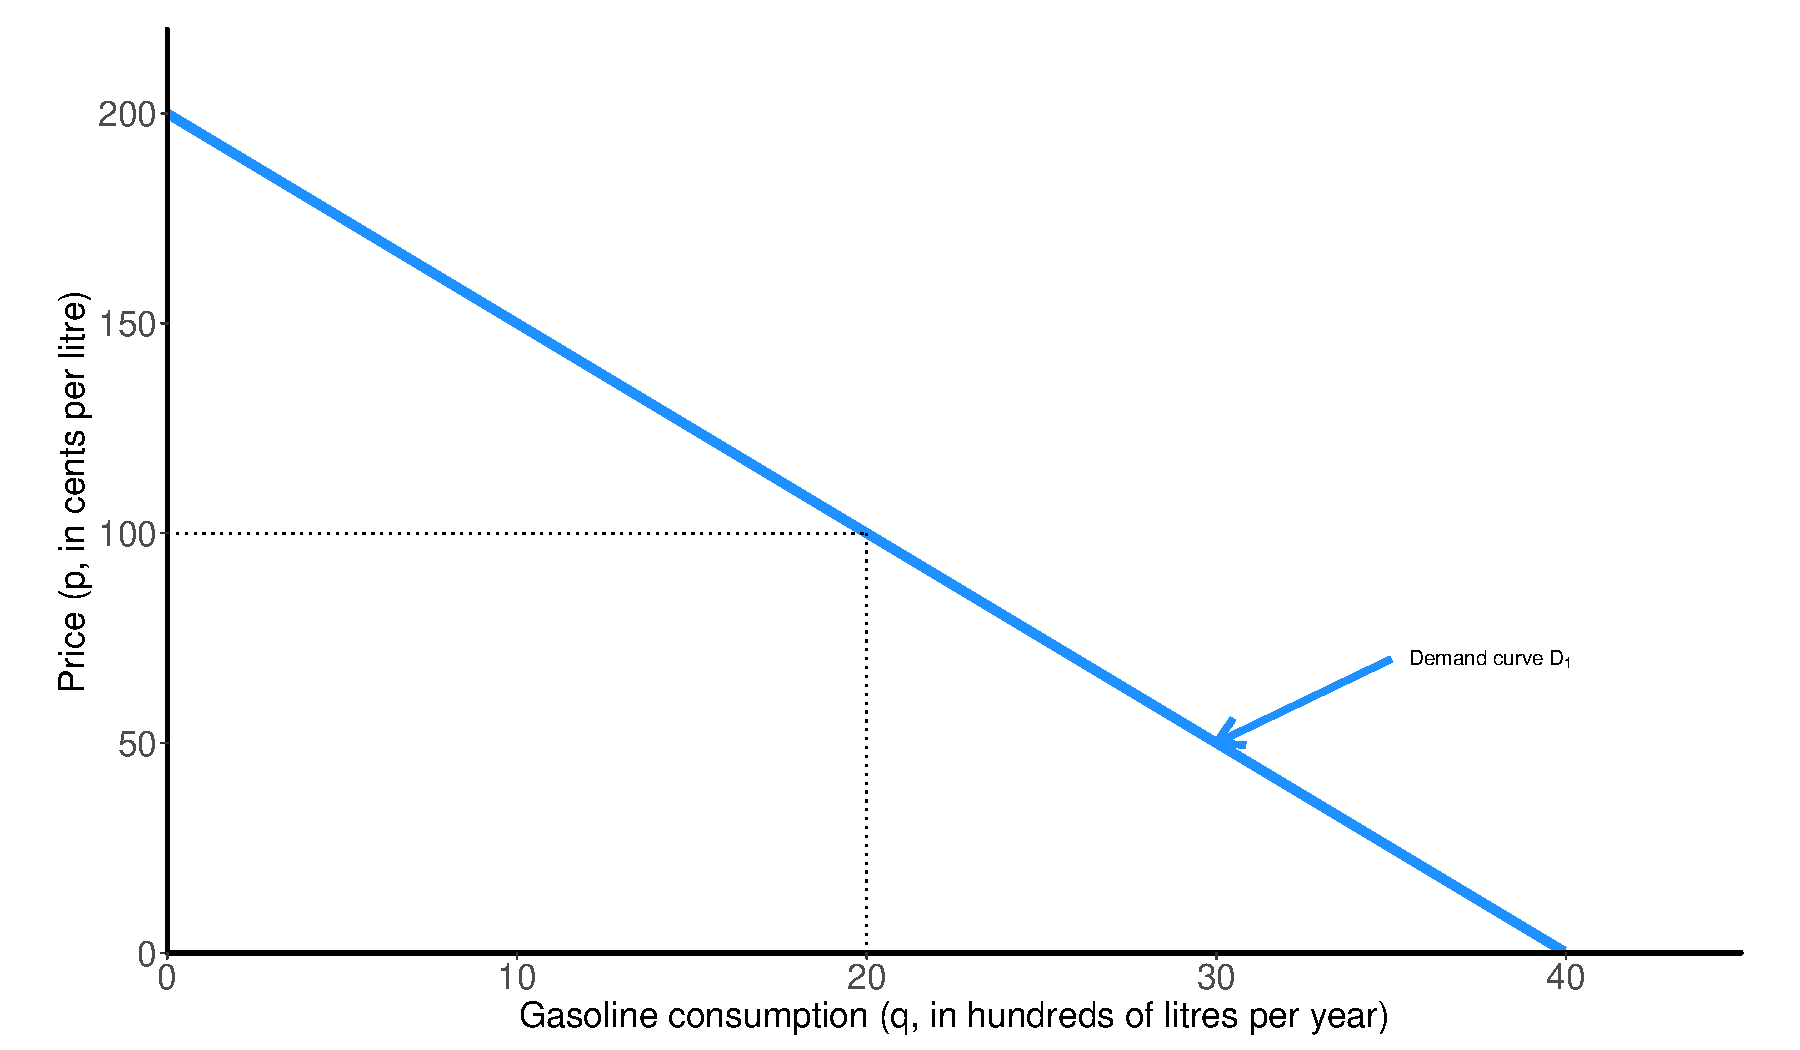
\includegraphics{estimation_deck_files/figure-beamer/demand_graph_1-1.pdf}
\end{frame}

\begin{frame}{Graph comparison}
\protect\hypertarget{graph-comparison-1}{}
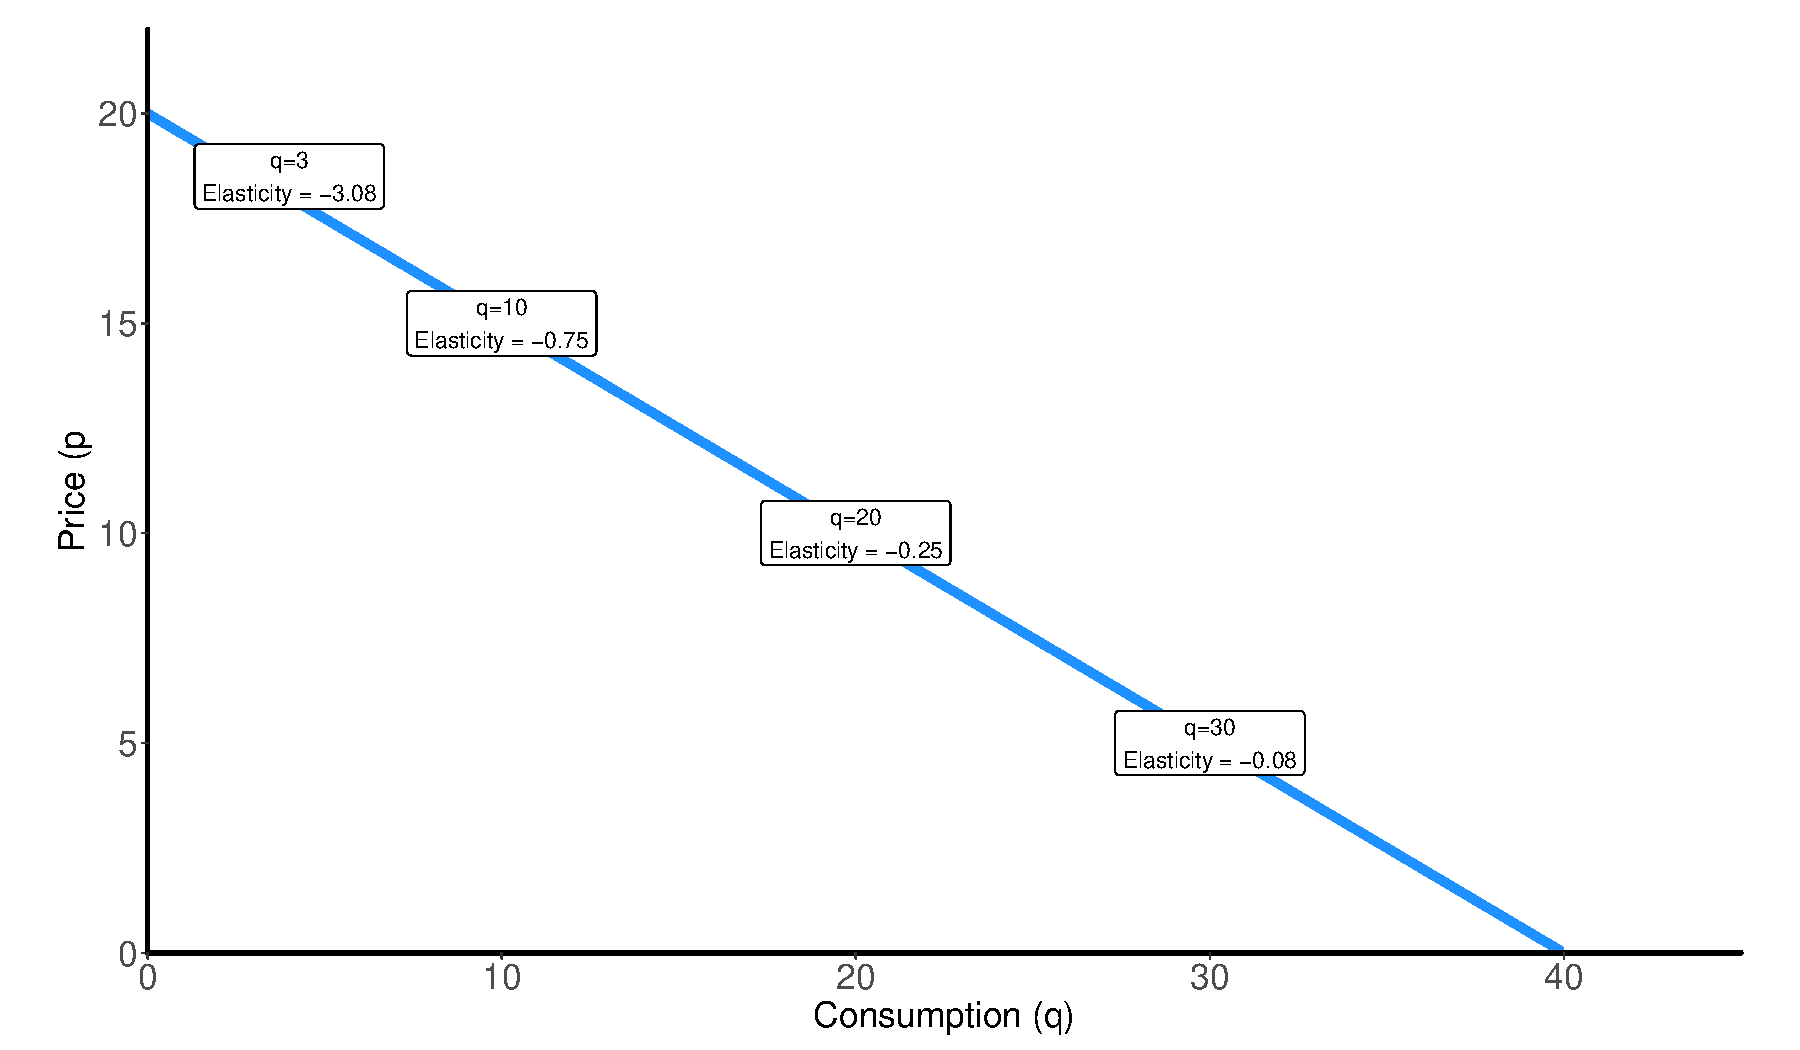
\includegraphics{estimation_deck_files/figure-beamer/demand_graph_2-1.pdf}
\end{frame}

\begin{frame}{Estimation of elasticities}
\protect\hypertarget{estimation-of-elasticities}{}
\begin{itemize}
\tightlist
\item
  We can use real world data to estimate elasticities
\item
  Examples:

  \begin{itemize}
  \tightlist
  \item
    Do emissions respond to carbon pricing? (BC carbon tax)
  \item
    Do wages affect labour supply? (Alberta's minimum wage changes)
  \item
    Do the prices of complements affect labour supply? (Quebec child
    care)
  \item
    Do changes in production technology or regulation affect supply (US
    light tight oil)
  \end{itemize}
\item
  Beware:

  \begin{itemize}
  \tightlist
  \item
    Correlation vs causation
  \item
    Omitted variables bias
  \item
    Sample selection bias
  \end{itemize}
\end{itemize}
\end{frame}

\begin{frame}{Estimation of demand}
\protect\hypertarget{estimation-of-demand}{}
What is a general manager paying for when they sign a hockey player?

\begin{itemize}
\tightlist
\item
  goals?
\item
  assists?
\item
  points?
\end{itemize}

What other attributes might matter the an orginization's willingness to
pay for a player?

\vfill
\end{frame}

\begin{frame}{You might have a sense of where this is going\ldots{}}
\protect\hypertarget{you-might-have-a-sense-of-where-this-is-going}{}
\url{https://www.nytimes.com/video/movies/100000001341145/clip-moneyball.html}
\end{frame}

\begin{frame}{Economic Moneyball}
\protect\hypertarget{economic-moneyball}{}
Much of the estimation of demand is trying to determine, with
statistical tools, the marginal willingness to pay for just one more:

\begin{itemize}
\tightlist
\item
  run
\item
  year of education
\item
  year of experience
\item
  goal
\item
  square footage of floor space
\item
  tenth of a point of GPA
\item
  horsepower
\item
  kWh
\item
  hour of work
\end{itemize}
\end{frame}

\begin{frame}{Economic Moneyball}
\protect\hypertarget{economic-moneyball-1}{}
Much of the estimation of demand is trying to determine, with
statistical tolls, the marginal willingness to pay for just one more:

\begin{itemize}
\tightlist
\item
  run (SABR-metrics)
\item
  year of education (human capital)
\item
  year of experience (human capital)
\item
  goal (hockey analytics)
\item
  square footage of floor space (real estate)
\item
  tenth of a point of GPA (labour markets)
\item
  horsepower (vehicle pricing)
\item
  kWh (vehicle pricing)
\item
  hour of work (labour markets)
\end{itemize}
\end{frame}

\begin{frame}{Let's try a couple out}
\protect\hypertarget{lets-try-a-couple-out}{}
\begin{itemize}
\tightlist
\item
  Start with NHL hockey salaries and performance statistics from the
  2018-2019 season \url{https://www.capfriendly.com/}
\item
  Choose only players making more than \$1 million per year
\item
  Build a model for the willingness to pay based on salaries as a
  function of performance
\end{itemize}
\end{frame}

\begin{frame}{A basic, univariate regression}
\protect\hypertarget{a-basic-univariate-regression}{}
\vspace{-.5cm}

\begin{table}[!htbp] \centering 
  \caption{NHL Salary Regression Models} 
  \label{} 
\tiny 
\begin{tabular}{@{\extracolsep{5pt}}lD{.}{.}{-3} } 
\\[-1.8ex]\hline 
\hline \\[-1.8ex] 
 & \multicolumn{1}{c}{\textit{Dependent variable:}} \\ 
\cline{2-2} 
\\[-1.8ex] & \multicolumn{1}{c}{salary} \\ 
\hline \\[-1.8ex] 
 Constant & 1.840^{***}$ $(0.176) \\ 
  points & 0.065^{***}$ $(0.004) \\ 
 \hline \\[-1.8ex] 
Observations & \multicolumn{1}{c}{440} \\ 
Adjusted R$^{2}$ & \multicolumn{1}{c}{0.354} \\ 
Residual Std. Error & \multicolumn{1}{c}{2.090 (df = 438)} \\ 
\hline 
\hline \\[-1.8ex] 
\textit{Note:}  & \multicolumn{1}{r}{$^{*}$p$<$0.1; $^{**}$p$<$0.05; $^{***}$p$<$0.01} \\ 
\end{tabular} 
\end{table}

\begin{itemize}
\tightlist
\item
  The regression tells us that the average salary is \$1.845 million
  with \textit{one more point} being worth \$65,372.400, the precise
  value of the reported coefficient on points, 0.065, converted to
  thousands of dollars. \vfill
\end{itemize}
\end{frame}

\begin{frame}{A basic, univariate regression}
\protect\hypertarget{a-basic-univariate-regression-1}{}
\vspace{-.5cm}

\begin{table}[!htbp] \centering 
  \caption{NHL Salary Regression Models} 
  \label{} 
\tiny 
\begin{tabular}{@{\extracolsep{5pt}}lD{.}{.}{-3} } 
\\[-1.8ex]\hline 
\hline \\[-1.8ex] 
 & \multicolumn{1}{c}{\textit{Dependent variable:}} \\ 
\cline{2-2} 
\\[-1.8ex] & \multicolumn{1}{c}{salary} \\ 
\hline \\[-1.8ex] 
 Constant & 1.840^{***}$ $(0.176) \\ 
  points & 0.065^{***}$ $(0.004) \\ 
 \hline \\[-1.8ex] 
Observations & \multicolumn{1}{c}{440} \\ 
Adjusted R$^{2}$ & \multicolumn{1}{c}{0.354} \\ 
Residual Std. Error & \multicolumn{1}{c}{2.090 (df = 438)} \\ 
\hline 
\hline \\[-1.8ex] 
\textit{Note:}  & \multicolumn{1}{r}{$^{*}$p$<$0.1; $^{**}$p$<$0.05; $^{***}$p$<$0.01} \\ 
\end{tabular} 
\end{table}

\begin{itemize}
\tightlist
\item
  The standard errors tell us how precisely the coefficients are
  estimated. A consistent relationship or a larger sample size will give
  you smaller standard errors.
\item
  The regression tells us that \textit{one more point} is worth
  \$65,372.403 \(\pm\) \$8,242.740, 19 times out of 20.
\end{itemize}

\vfill
\end{frame}

\begin{frame}{Graph comparison}
\protect\hypertarget{graph-comparison-2}{}
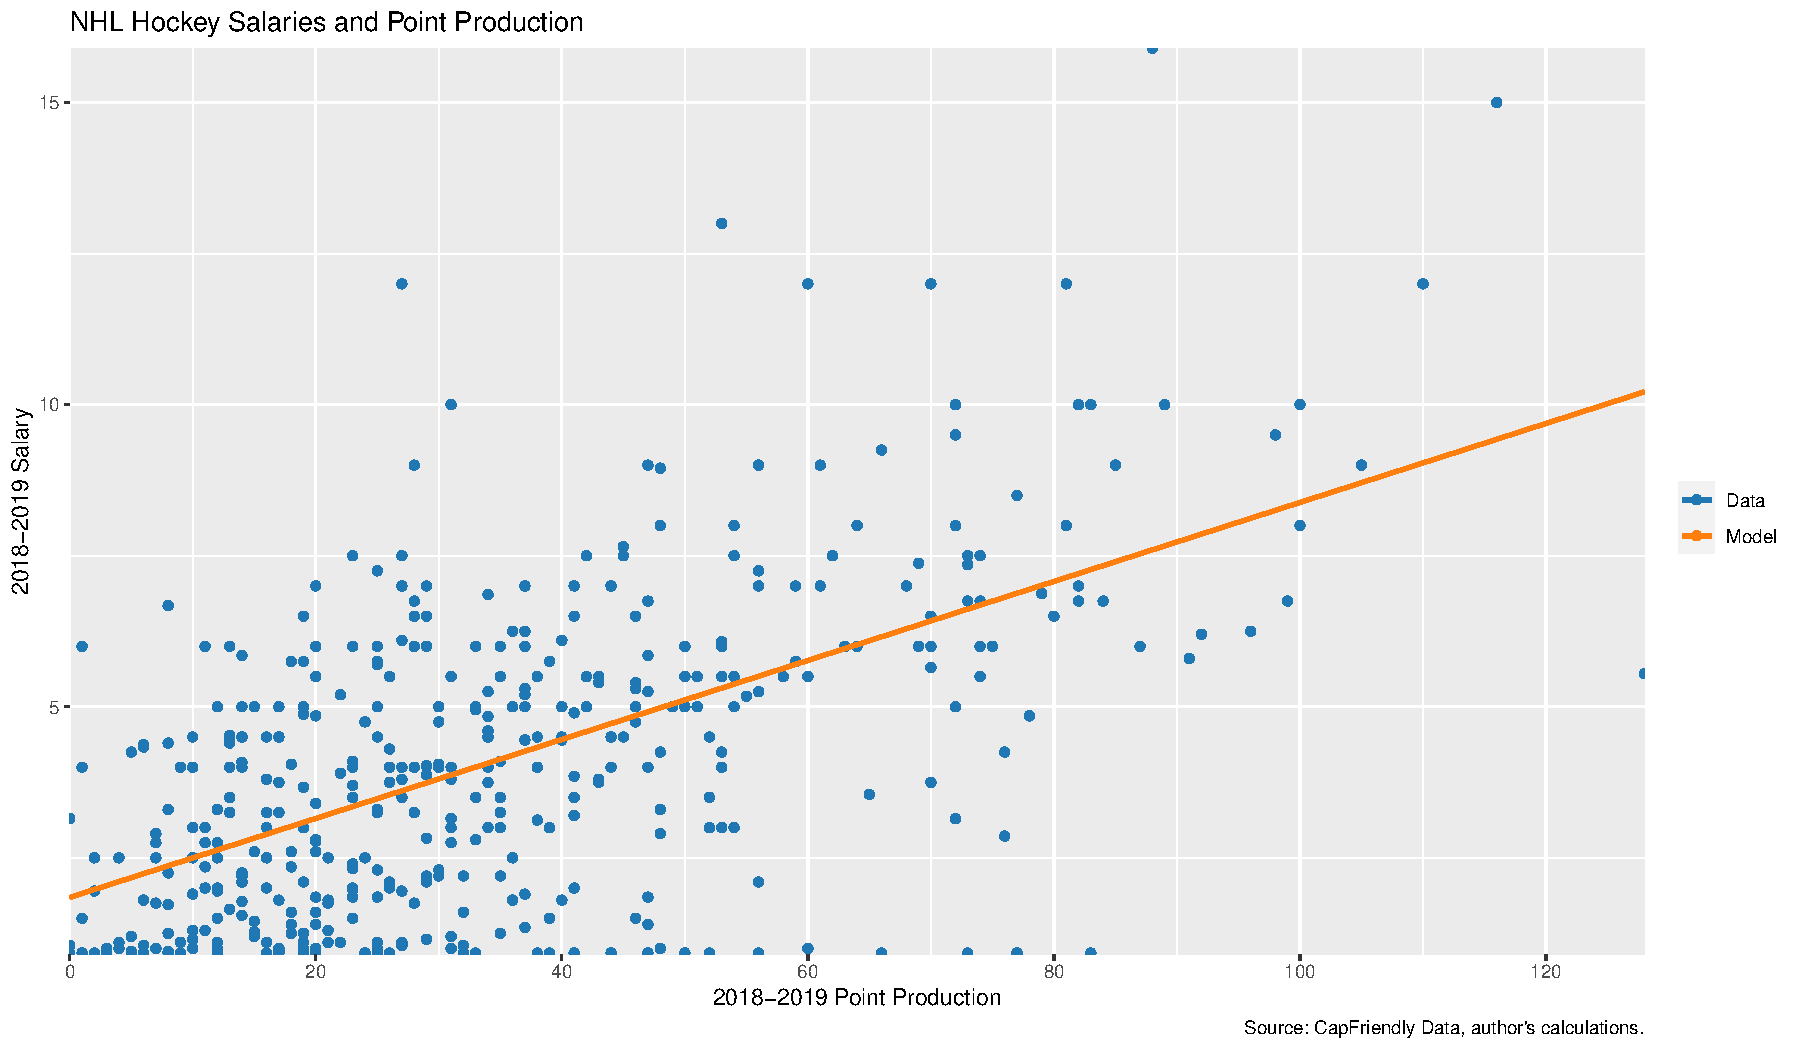
\includegraphics{estimation_deck_files/figure-beamer/nhl_salary_graph-1.pdf}
\end{frame}

\begin{frame}{Goodness of fit}
\protect\hypertarget{goodness-of-fit}{}
\begin{itemize}
\tightlist
\item
  R-squared (\(R^2\)) statistic measures the goodness of fit, or the
  share of the variation in the dependent variable (salary) that is
  explained by the regression.
\item
  The statistic must lie between 0 and 1.

  \begin{itemize}
  \tightlist
  \item
    1 indicates that 100\% of the variation is explained by the
    regression.
  \end{itemize}
\item
  Adjusted R-squared is a modified version of R-squared

  \begin{itemize}
  \tightlist
  \item
    Adjusted for the number of predictors in the model.
  \item
    The adjusted R-squared increases only if the new term improves the
    model more than would be expected by chance.
  \end{itemize}
\item
  \(R^2=1-\frac{SS_{Res}}{SS_{Total}}\), where \(SS_{Res}\) and
  \(SS_{Total}\) are the sum of squared residuals and total dependent
  variable sum of squares.
\item
  \(Adj\,R^2=1- \frac{(1-R^2)(n-1)}{n-k-1}\), where k is the number of
  parameters.
\end{itemize}
\end{frame}

\begin{frame}{Residuals and what they can tell us}
\protect\hypertarget{residuals-and-what-they-can-tell-us}{}
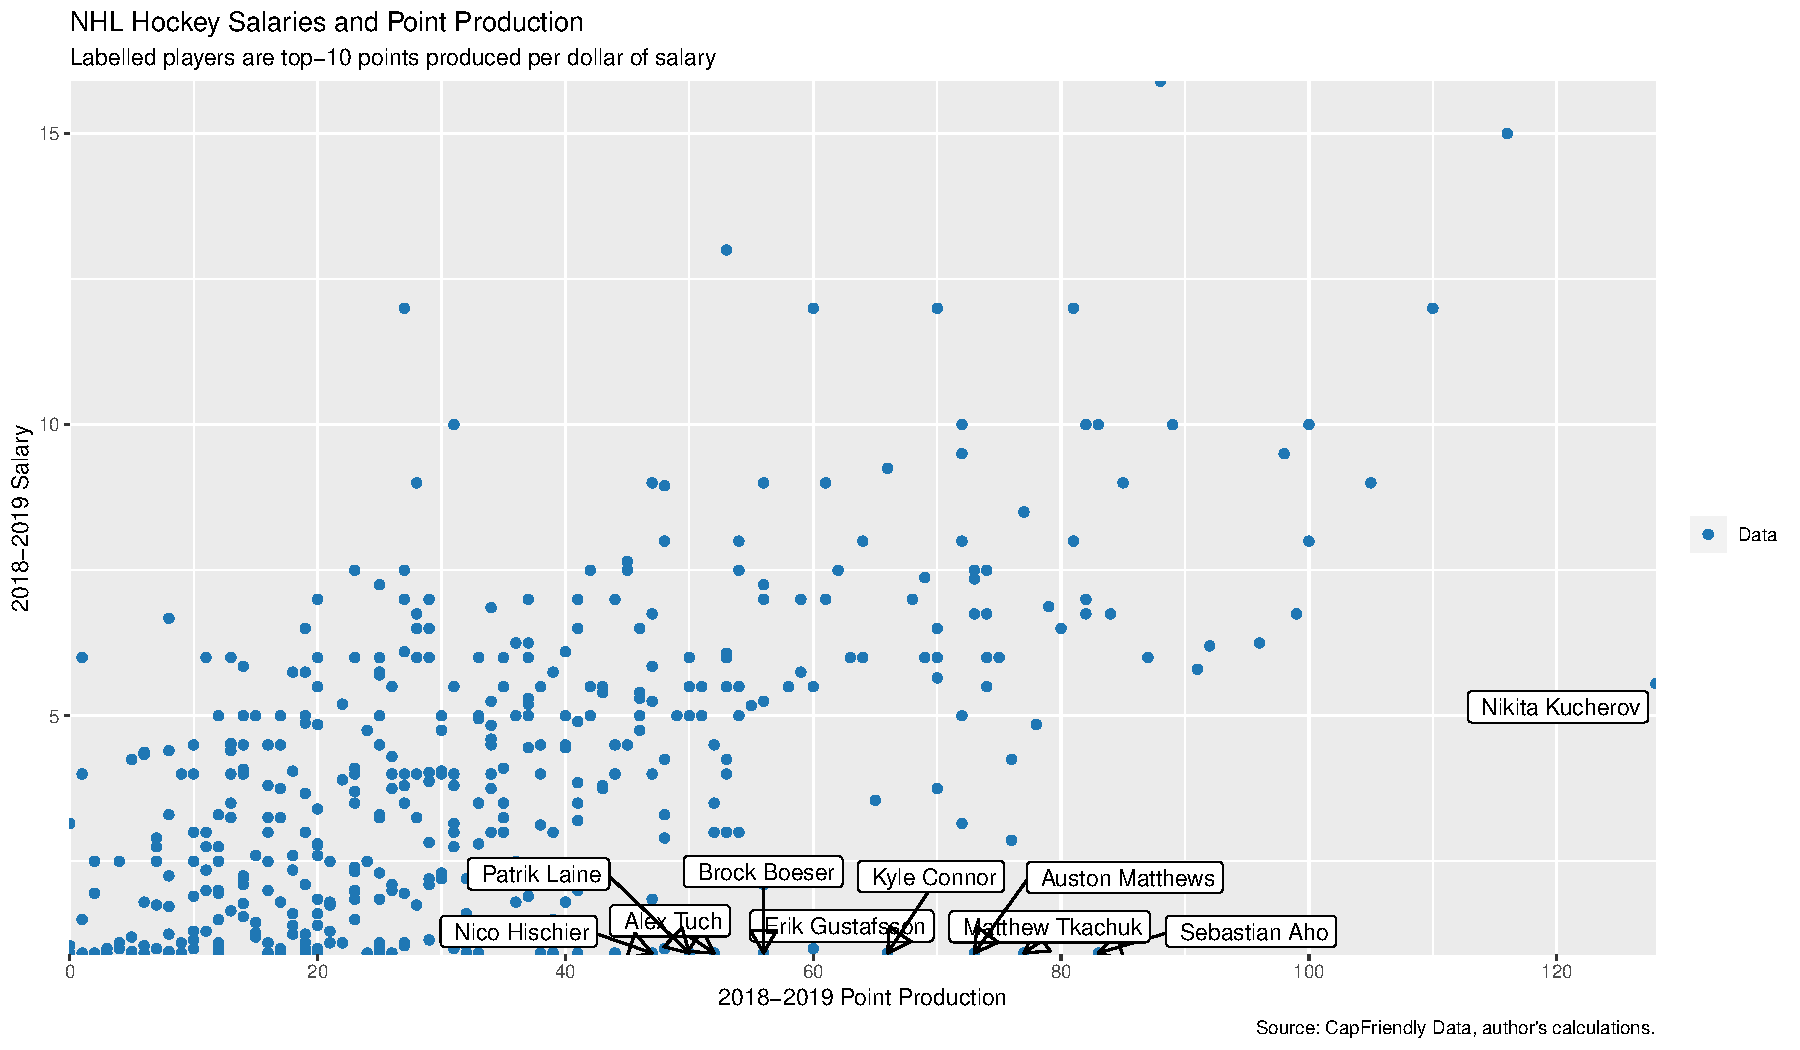
\includegraphics{estimation_deck_files/figure-beamer/nhl_residuals_graph-1.pdf}
\end{frame}

\begin{frame}{Now who are the most underpaid players?}
\protect\hypertarget{now-who-are-the-most-underpaid-players}{}
\begin{table}[!htbp] \centering 
  \caption{} 
  \label{} 
\small 
\begin{tabular}{@{\extracolsep{5pt}} c} 
\\[-1.8ex]\hline 
\hline \\[-1.8ex] 
label \\ 
\hline \\[-1.8ex] 
\#1:  Sebastian Aho \\ 
\#2:  Matthew Tkachuk \\ 
\#3:  Auston Matthews \\ 
\#4:  Kyle Connor \\ 
\#5:  Erik Gustafsson \\ 
\#6:  Nikita Kucherov \\ 
\#7:  Brock Boeser \\ 
\#8:  Alex Tuch \\ 
\#9:  Patrik Laine \\ 
\#10:  Nico Hischier \\ 
\hline \\[-1.8ex] 
\end{tabular} 
\end{table} 
\vfill
\end{frame}

\begin{frame}{What are we missing}
\protect\hypertarget{what-are-we-missing}{}
\begin{itemize}
\tightlist
\item
  Multivariate regression
\item
  Sample selection bias
\item
  Omitted variables bias
\item
  Causality vs correlation
\end{itemize}
\end{frame}

\begin{frame}{Multivariate regression}
\protect\hypertarget{multivariate-regression}{}
\begin{itemize}
\tightlist
\item
  Multivariate Regression uses two or more explanatory variables.

  \begin{itemize}
  \tightlist
  \item
    e.g.~\(s = a + b X_1 + cX_2 + \epsilon\).
  \end{itemize}
\item
  We can estimate (in our case) NHL salaries as a function of point
  production but also other explanatory variables

  \begin{itemize}
  \tightlist
  \item
    a, b, and c are \textbf{coefficients} to be estimated
  \item
    \(\epsilon\) is a random error or residual.
  \end{itemize}
\item
  When we use least squares regression to estimate a, b, and c, we get a
  prediction of the salary for combination of measurable outputs.
\item
  Least squares regression minimizes the sum of squared residuals.

  \begin{itemize}
  \tightlist
  \item
    We can also learn from residuals
  \end{itemize}
\item
  With multivariate regression, we can isolate the individual
  \textbf{marginal effects} of each explanatory variable
  \textbf{holding the other explanatory variables constant}.
\end{itemize}
\end{frame}

\begin{frame}{A slightly better regression}
\protect\hypertarget{a-slightly-better-regression}{}
\vspace{-.5cm}

\begin{table}[!htbp] \centering 
  \caption{NHL Salary Regression Models} 
  \label{} 
\tiny 
\begin{tabular}{@{\extracolsep{-15pt}}lD{.}{.}{-3} D{.}{.}{-3} } 
\\[-1.8ex]\hline 
\hline \\[-1.8ex] 
 & \multicolumn{2}{c}{\textit{Dependent variable:}} \\ 
\cline{2-3} 
\\[-1.8ex] & \multicolumn{2}{c}{salary} \\ 
\\[-1.8ex] & \multicolumn{1}{c}{(1)} & \multicolumn{1}{c}{(2)}\\ 
\hline \\[-1.8ex] 
 Constant & 1.840^{***}$ $(0.176) & -1.220^{***}$ $(0.460) \\ 
  points & 0.065^{***}$ $(0.004) & 0.050^{***}$ $(0.005) \\ 
  toi &  & 0.206^{***}$ $(0.029) \\ 
 \hline \\[-1.8ex] 
Observations & \multicolumn{1}{c}{440} & \multicolumn{1}{c}{440} \\ 
Adjusted R$^{2}$ & \multicolumn{1}{c}{0.354} & \multicolumn{1}{c}{0.420} \\ 
Residual Std. Error & \multicolumn{1}{c}{2.090 (df = 438)} & \multicolumn{1}{c}{1.980 (df = 437)} \\ 
\hline 
\hline \\[-1.8ex] 
\textit{Note:}  & \multicolumn{2}{r}{$^{*}$p$<$0.1; $^{**}$p$<$0.05; $^{***}$p$<$0.01} \\ 
\end{tabular} 
\end{table}

\begin{itemize}
\tightlist
\item
  The second regression tells us that the unadjusted salary is \$-1.219
  million with \textit{one more point} being worth \$50,411.400, and
  \textit{one more minute of ice time} being worth \$205,631.820.
\item
  How can a negative unadjusted salary value possibly make sense? Have I
  done something wrong? \vfill
\end{itemize}
\end{frame}

\begin{frame}{Now who are the most underpaid players?}
\protect\hypertarget{now-who-are-the-most-underpaid-players-1}{}
\begin{table}[!htbp] \centering 
  \caption{} 
  \label{} 
\small 
\begin{tabular}{@{\extracolsep{5pt}} c} 
\\[-1.8ex]\hline 
\hline \\[-1.8ex] 
label \\ 
\hline \\[-1.8ex] 
\#1:  Sebastian Aho \\ 
\#2:  Erik Gustafsson \\ 
\#3:  Matthew Tkachuk \\ 
\#4:  Auston Matthews \\ 
\#5:  Kyle Connor \\ 
\#6:  Zachary Werenski \\ 
\#7:  Brock Boeser \\ 
\#8:  Nico Hischier \\ 
\#9:  Patrik Laine \\ 
\#10:  Alex Tuch \\ 
\hline \\[-1.8ex] 
\end{tabular} 
\end{table} 
\vfill
\end{frame}

\begin{frame}{Now who are the most underpaid players?}
\protect\hypertarget{now-who-are-the-most-underpaid-players-2}{}
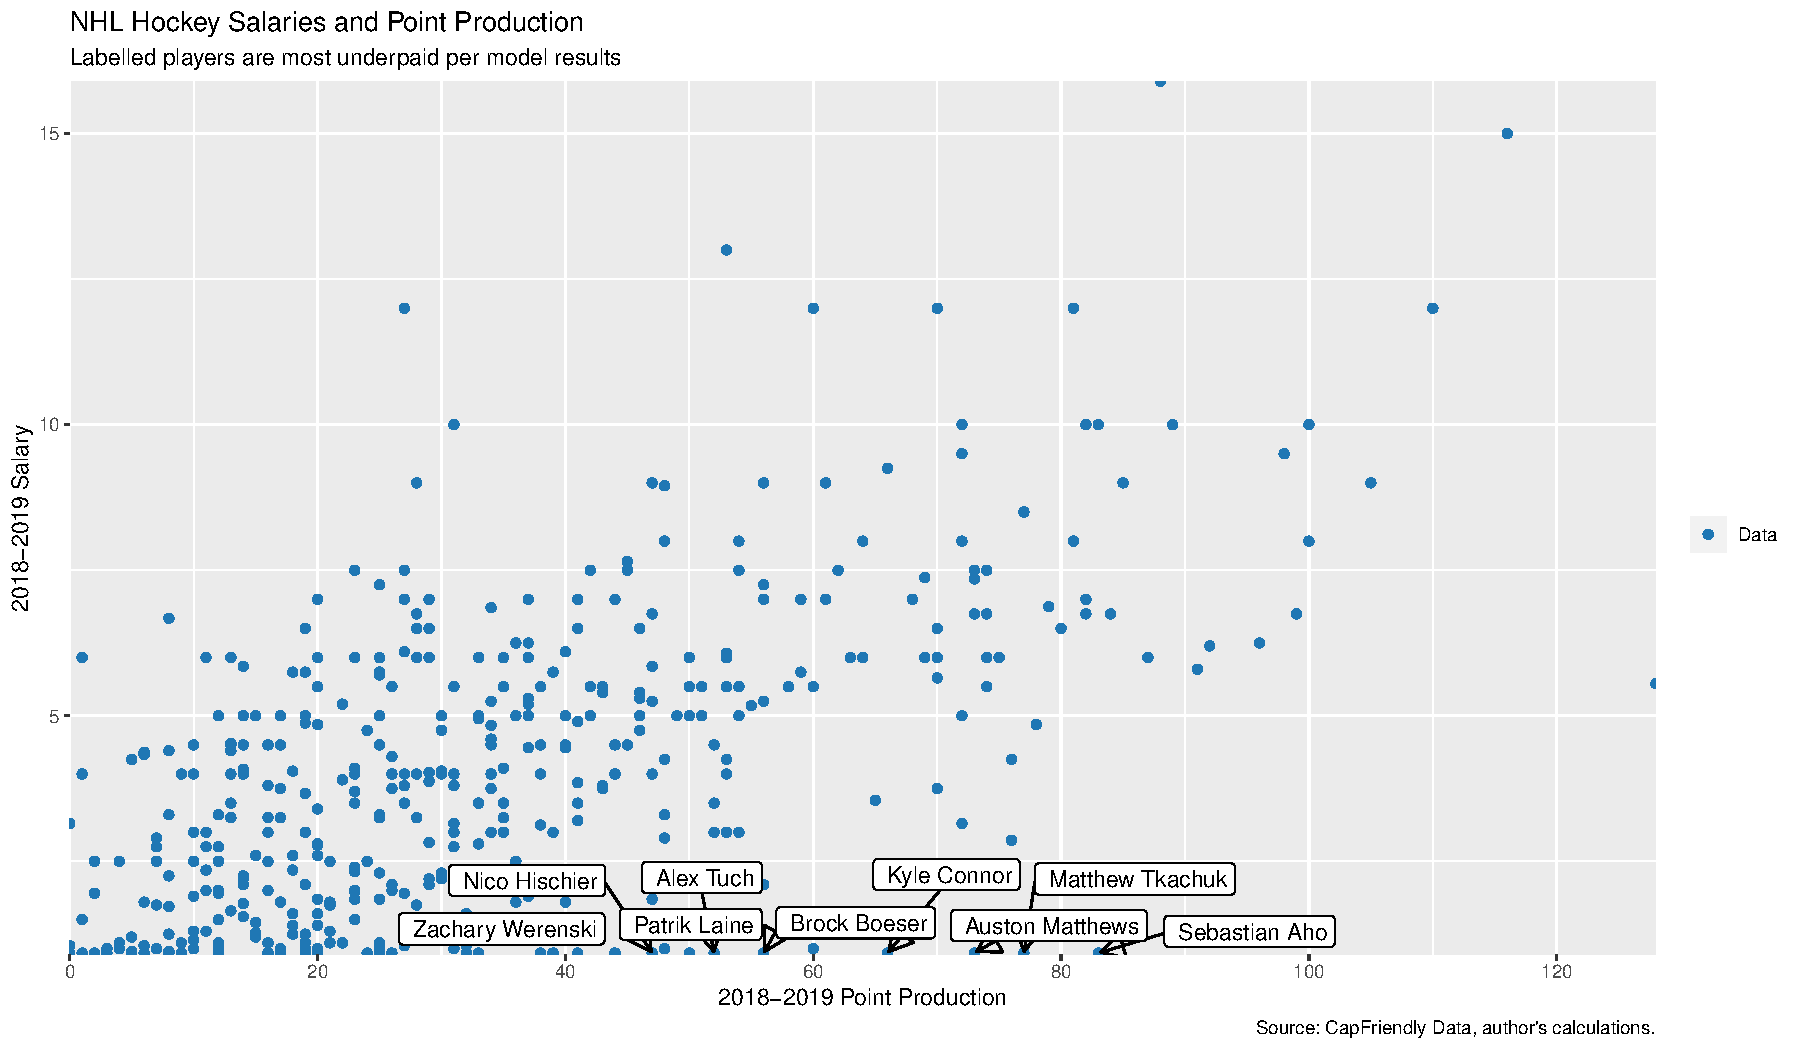
\includegraphics{estimation_deck_files/figure-beamer/nhl_residuals_graph_2-1.pdf}
\end{frame}

\begin{frame}{Adjust for position}
\protect\hypertarget{adjust-for-position}{}
\vspace{-.5cm}

\begin{table}[!htbp] \centering 
  \caption{NHL Salary Regression Models} 
  \label{} 
\tiny 
\begin{tabular}{@{\extracolsep{-15pt}}lD{.}{.}{-3} D{.}{.}{-3} D{.}{.}{-3} } 
\\[-1.8ex]\hline 
\hline \\[-1.8ex] 
 & \multicolumn{3}{c}{\textit{Dependent variable:}} \\ 
\cline{2-4} 
\\[-1.8ex] & \multicolumn{3}{c}{salary} \\ 
\\[-1.8ex] & \multicolumn{1}{c}{(1)} & \multicolumn{1}{c}{(2)} & \multicolumn{1}{c}{(3)}\\ 
\hline \\[-1.8ex] 
 Constant & 1.840^{***}$ $(0.176) & -1.220^{***}$ $(0.460) & -2.290^{***}$ $(0.810) \\ 
  points & 0.065^{***}$ $(0.004) & 0.050^{***}$ $(0.005) & 0.038^{***}$ $(0.008) \\ 
  toi &  & 0.206^{***}$ $(0.029) & 0.309^{***}$ $(0.066) \\ 
  positionD &  &  & -0.575$ $(1.630) \\ 
  toi:positionD &  &  & -0.011$ $(0.106) \\ 
  points:positionD &  &  & -0.003$ $(0.017) \\ 
 \hline \\[-1.8ex] 
Observations & \multicolumn{1}{c}{440} & \multicolumn{1}{c}{440} & \multicolumn{1}{c}{440} \\ 
Adjusted R$^{2}$ & \multicolumn{1}{c}{0.354} & \multicolumn{1}{c}{0.420} & \multicolumn{1}{c}{0.423} \\ 
Residual Std. Error & \multicolumn{1}{c}{2.090 (df = 438)} & \multicolumn{1}{c}{1.980 (df = 437)} & \multicolumn{1}{c}{1.970 (df = 434)} \\ 
\hline 
\hline \\[-1.8ex] 
\textit{Note:}  & \multicolumn{3}{r}{$^{*}$p$<$0.1; $^{**}$p$<$0.05; $^{***}$p$<$0.01} \\ 
\end{tabular} 
\end{table}

\begin{itemize}
\tightlist
\item
  The third regression tells us that the unadjusted salary is \$-2.289
  million with \textit{one more point} being worth \$38,245.700, and
  \textit{one more minute of ice time} being worth \$38,245.700.
\item
  We also adjust for differential values for each for defence vs
  forwards.
\end{itemize}
\end{frame}

\begin{frame}{Adjust for position}
\protect\hypertarget{adjust-for-position-1}{}
\vspace{-.5cm}

\begin{table}[!htbp] \centering 
  \caption{NHL Salary Regression Models} 
  \label{} 
\tiny 
\begin{tabular}{@{\extracolsep{-15pt}}lD{.}{.}{-3} D{.}{.}{-3} D{.}{.}{-3} } 
\\[-1.8ex]\hline 
\hline \\[-1.8ex] 
 & \multicolumn{3}{c}{\textit{Dependent variable:}} \\ 
\cline{2-4} 
\\[-1.8ex] & \multicolumn{3}{c}{salary} \\ 
\\[-1.8ex] & \multicolumn{1}{c}{(1)} & \multicolumn{1}{c}{(2)} & \multicolumn{1}{c}{(3)}\\ 
\hline \\[-1.8ex] 
 Constant & 1.840^{***}$ $(0.176) & -1.220^{***}$ $(0.460) & -2.290^{***}$ $(0.810) \\ 
  points & 0.065^{***}$ $(0.004) & 0.050^{***}$ $(0.005) & 0.038^{***}$ $(0.008) \\ 
  toi &  & 0.206^{***}$ $(0.029) & 0.309^{***}$ $(0.066) \\ 
  positionD &  &  & -0.575$ $(1.630) \\ 
  toi:positionD &  &  & -0.011$ $(0.106) \\ 
  points:positionD &  &  & -0.003$ $(0.017) \\ 
 \hline \\[-1.8ex] 
Observations & \multicolumn{1}{c}{440} & \multicolumn{1}{c}{440} & \multicolumn{1}{c}{440} \\ 
Adjusted R$^{2}$ & \multicolumn{1}{c}{0.354} & \multicolumn{1}{c}{0.420} & \multicolumn{1}{c}{0.423} \\ 
Residual Std. Error & \multicolumn{1}{c}{2.090 (df = 438)} & \multicolumn{1}{c}{1.980 (df = 437)} & \multicolumn{1}{c}{1.970 (df = 434)} \\ 
\hline 
\hline \\[-1.8ex] 
\textit{Note:}  & \multicolumn{3}{r}{$^{*}$p$<$0.1; $^{**}$p$<$0.05; $^{***}$p$<$0.01} \\ 
\end{tabular} 
\end{table}

\begin{itemize}
\tightlist
\item
  Note here that, as we add variables to the regression which help
  explain the salary levels, we're seeing the other coefficient values
  change. Why?
\end{itemize}

\vfill
\end{frame}

\begin{frame}{Now who are the most underpaid players?}
\protect\hypertarget{now-who-are-the-most-underpaid-players-3}{}
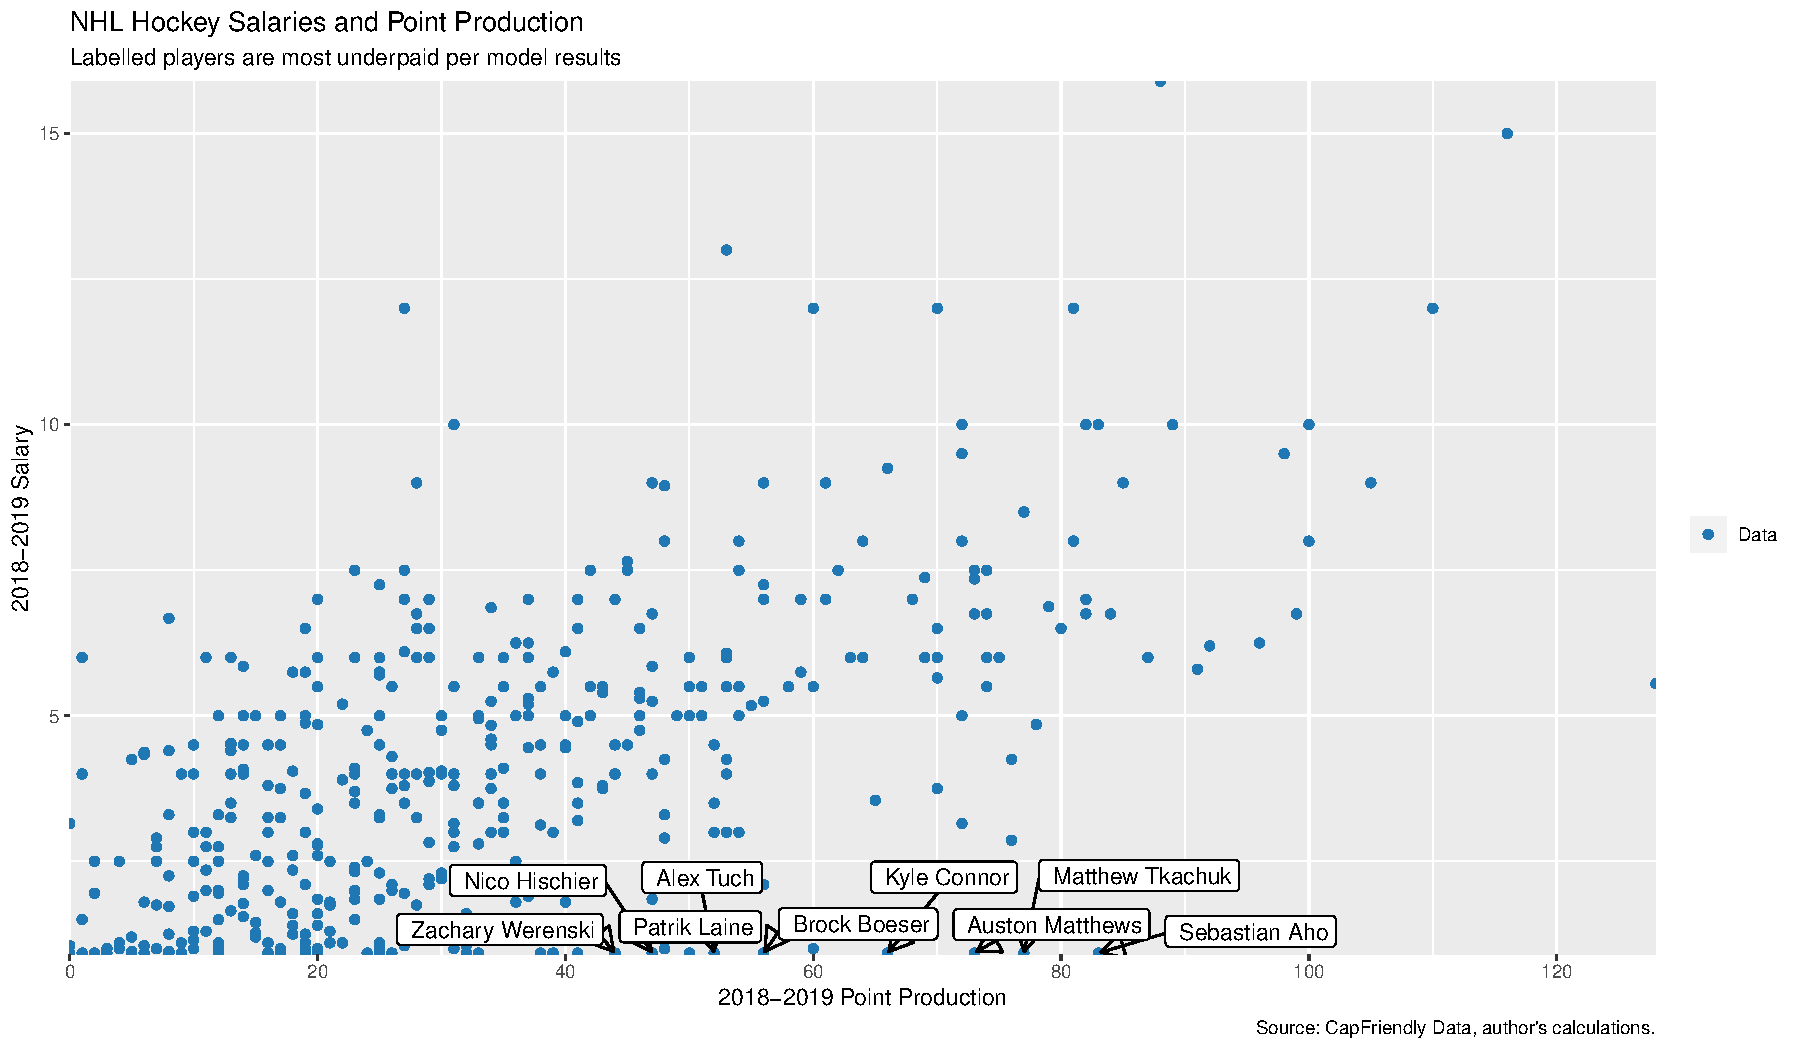
\includegraphics{estimation_deck_files/figure-beamer/nhl_residuals_graph_3-1.pdf}
\vfill
\end{frame}

\begin{frame}{Now who are the most underpaid players?}
\protect\hypertarget{now-who-are-the-most-underpaid-players-4}{}
\begin{table}[!htbp] \centering 
  \caption{} 
  \label{} 
\small 
\begin{tabular}{@{\extracolsep{5pt}} c} 
\\[-1.8ex]\hline 
\hline \\[-1.8ex] 
label \\ 
\hline \\[-1.8ex] 
\#1:  Sebastian Aho \\ 
\#2:  Auston Matthews \\ 
\#3:  Kyle Connor \\ 
\#4:  Matthew Tkachuk \\ 
\#5:  Erik Gustafsson \\ 
\#6:  Brock Boeser \\ 
\#7:  Zachary Werenski \\ 
\#8:  Nico Hischier \\ 
\#9:  Patrik Laine \\ 
\#10:  Alex Tuch \\ 
\hline \\[-1.8ex] 
\end{tabular} 
\end{table} 
\vfill
\end{frame}

\begin{frame}{Omitted variables bias}
\protect\hypertarget{omitted-variables-bias}{}
\vspace{-.5cm}

\begin{table}[!htbp] \centering 
  \caption{NHL Salary Regression Models} 
  \label{} 
\tiny 
\begin{tabular}{@{\extracolsep{-15pt}}lD{.}{.}{-3} D{.}{.}{-3} D{.}{.}{-3} } 
\\[-1.8ex]\hline 
\hline \\[-1.8ex] 
 & \multicolumn{3}{c}{\textit{Dependent variable:}} \\ 
\cline{2-4} 
\\[-1.8ex] & \multicolumn{3}{c}{salary} \\ 
\\[-1.8ex] & \multicolumn{1}{c}{(1)} & \multicolumn{1}{c}{(2)} & \multicolumn{1}{c}{(3)}\\ 
\hline \\[-1.8ex] 
 Constant & 1.840^{***}$ $(0.176) & -1.220^{***}$ $(0.460) & -2.290^{***}$ $(0.810) \\ 
  points & 0.065^{***}$ $(0.004) & 0.050^{***}$ $(0.005) & 0.038^{***}$ $(0.008) \\ 
  toi &  & 0.206^{***}$ $(0.029) & 0.309^{***}$ $(0.066) \\ 
  positionD &  &  & -0.575$ $(1.630) \\ 
  toi:positionD &  &  & -0.011$ $(0.106) \\ 
  points:positionD &  &  & -0.003$ $(0.017) \\ 
 \hline \\[-1.8ex] 
Observations & \multicolumn{1}{c}{440} & \multicolumn{1}{c}{440} & \multicolumn{1}{c}{440} \\ 
Adjusted R$^{2}$ & \multicolumn{1}{c}{0.354} & \multicolumn{1}{c}{0.420} & \multicolumn{1}{c}{0.423} \\ 
Residual Std. Error & \multicolumn{1}{c}{2.090 (df = 438)} & \multicolumn{1}{c}{1.980 (df = 437)} & \multicolumn{1}{c}{1.970 (df = 434)} \\ 
\hline 
\hline \\[-1.8ex] 
\textit{Note:}  & \multicolumn{3}{r}{$^{*}$p$<$0.1; $^{**}$p$<$0.05; $^{***}$p$<$0.01} \\ 
\end{tabular} 
\end{table}

\begin{itemize}
\tightlist
\item
  In regression (1), I tried to explain salaries using only points. What
  variables did I omit?
\item
  TOI is obviously important, and so by omitting it, I'd been forcing
  points to explain other things that are correlated with it
\end{itemize}

\vfill
\end{frame}

\begin{frame}{Non-linear effects}
\protect\hypertarget{non-linear-effects}{}
\vspace{-.5cm}

\begin{table}[!htbp] \centering 
  \caption{NHL Salary Regression Models} 
  \label{} 
\tiny 
\begin{tabular}{@{\extracolsep{-15pt}}lD{.}{.}{-3} D{.}{.}{-3} D{.}{.}{-3} } 
\\[-1.8ex]\hline 
\hline \\[-1.8ex] 
 & \multicolumn{3}{c}{\textit{Dependent variable:}} \\ 
\cline{2-4} 
\\[-1.8ex] & \multicolumn{3}{c}{salary} \\ 
\\[-1.8ex] & \multicolumn{1}{c}{(1)} & \multicolumn{1}{c}{(2)} & \multicolumn{1}{c}{(3)}\\ 
\hline \\[-1.8ex] 
 Constant & 1.840^{***}$ $(0.176) & -1.220^{***}$ $(0.460) & -1.220^{***}$ $(0.460) \\ 
  points & 0.065^{***}$ $(0.004) & 0.050^{***}$ $(0.005) & 0.050^{***}$ $(0.005) \\ 
  toi &  & 0.206^{***}$ $(0.029) & 0.206^{***}$ $(0.029) \\ 
 \hline \\[-1.8ex] 
Observations & \multicolumn{1}{c}{440} & \multicolumn{1}{c}{440} & \multicolumn{1}{c}{440} \\ 
Adjusted R$^{2}$ & \multicolumn{1}{c}{0.354} & \multicolumn{1}{c}{0.420} & \multicolumn{1}{c}{0.420} \\ 
Residual Std. Error & \multicolumn{1}{c}{2.090 (df = 438)} & \multicolumn{1}{c}{1.980 (df = 437)} & \multicolumn{1}{c}{1.980 (df = 437)} \\ 
\hline 
\hline \\[-1.8ex] 
\textit{Note:}  & \multicolumn{3}{r}{$^{*}$p$<$0.1; $^{**}$p$<$0.05; $^{***}$p$<$0.01} \\ 
\end{tabular} 
\end{table}

\begin{itemize}
\tightlist
\item
  Note here that, as we add variables to the regression which help
  explain the salary levels, we're allowing for non-linear effects of
  points or toi. Why?
\end{itemize}

\vfill
\end{frame}

\begin{frame}{Omitted variables bias}
\protect\hypertarget{omitted-variables-bias-1}{}
\vspace{-.5cm}

\begin{table}[!htbp] \centering 
  \caption{NHL Salary Regression Models} 
  \label{} 
\tiny 
\begin{tabular}{@{\extracolsep{-15pt}}lD{.}{.}{-3} D{.}{.}{-3} D{.}{.}{-3} } 
\\[-1.8ex]\hline 
\hline \\[-1.8ex] 
 & \multicolumn{3}{c}{\textit{Dependent variable:}} \\ 
\cline{2-4} 
\\[-1.8ex] & \multicolumn{3}{c}{salary} \\ 
\\[-1.8ex] & \multicolumn{1}{c}{(1)} & \multicolumn{1}{c}{(2)} & \multicolumn{1}{c}{(3)}\\ 
\hline \\[-1.8ex] 
 Constant & 1.840^{***}$ $(0.176) & -1.220^{***}$ $(0.460) & -2.290^{***}$ $(0.810) \\ 
  points & 0.065^{***}$ $(0.004) & 0.050^{***}$ $(0.005) & 0.038^{***}$ $(0.008) \\ 
  toi &  & 0.206^{***}$ $(0.029) & 0.309^{***}$ $(0.066) \\ 
  positionD &  &  & -0.575$ $(1.630) \\ 
  toi:positionD &  &  & -0.011$ $(0.106) \\ 
  points:positionD &  &  & -0.003$ $(0.017) \\ 
 \hline \\[-1.8ex] 
Observations & \multicolumn{1}{c}{440} & \multicolumn{1}{c}{440} & \multicolumn{1}{c}{440} \\ 
Adjusted R$^{2}$ & \multicolumn{1}{c}{0.354} & \multicolumn{1}{c}{0.420} & \multicolumn{1}{c}{0.423} \\ 
Residual Std. Error & \multicolumn{1}{c}{2.090 (df = 438)} & \multicolumn{1}{c}{1.980 (df = 437)} & \multicolumn{1}{c}{1.970 (df = 434)} \\ 
\hline 
\hline \\[-1.8ex] 
\textit{Note:}  & \multicolumn{3}{r}{$^{*}$p$<$0.1; $^{**}$p$<$0.05; $^{***}$p$<$0.01} \\ 
\end{tabular} 
\end{table}

\begin{itemize}
\tightlist
\item
  TOI is obviously important, and so by omitting it, I'd been forcing
  points to explain other things that are correlated with it like TOI
\item
  TOI, all else equal, correlates with points, so I was forcing points
  to explain both the direct (points) effect and the TOI (omitted)
  effect
\end{itemize}

\vfill
\end{frame}

\begin{frame}{Sample selection bias}
\protect\hypertarget{sample-selection-bias}{}
\vspace{-.5cm}

\begin{table}[!htbp] \centering 
  \caption{NHL Salary Regression Models} 
  \label{} 
\tiny 
\begin{tabular}{@{\extracolsep{-15pt}}lD{.}{.}{-3} D{.}{.}{-3} D{.}{.}{-3} } 
\\[-1.8ex]\hline 
\hline \\[-1.8ex] 
 & \multicolumn{3}{c}{\textit{Dependent variable:}} \\ 
\cline{2-4} 
\\[-1.8ex] & \multicolumn{3}{c}{salary} \\ 
\\[-1.8ex] & \multicolumn{1}{c}{(1)} & \multicolumn{1}{c}{(2)} & \multicolumn{1}{c}{(3)}\\ 
\hline \\[-1.8ex] 
 Constant & -1.220^{***}$ $(0.460) & 0.830$ $(0.551) & 3.190^{***}$ $(0.695) \\ 
  points & 0.050^{***}$ $(0.005) & 0.049^{***}$ $(0.004) & 0.041^{***}$ $(0.005) \\ 
  toi & 0.206^{***}$ $(0.029) & 0.130^{***}$ $(0.032) & 0.059$ $(0.037) \\ 
 \hline \\[-1.8ex] 
Observations & \multicolumn{1}{c}{440} & \multicolumn{1}{c}{324} & \multicolumn{1}{c}{223} \\ 
Adjusted R$^{2}$ & \multicolumn{1}{c}{0.420} & \multicolumn{1}{c}{0.379} & \multicolumn{1}{c}{0.287} \\ 
Residual Std. Error & \multicolumn{1}{c}{1.980 (df = 437)} & \multicolumn{1}{c}{1.770 (df = 321)} & \multicolumn{1}{c}{1.680 (df = 220)} \\ 
\hline 
\hline \\[-1.8ex] 
\textit{Note:}  & \multicolumn{3}{r}{$^{*}$p$<$0.1; $^{**}$p$<$0.05; $^{***}$p$<$0.01} \\ 
\end{tabular} 
\end{table}

\begin{itemize}
\tightlist
\item
  Regression (1) is players earning more than \$1 million, Regression
  (1) is players earning more than \$2 million, Regression (3) is
  players earning more than \$4 million.
\item
  The estimated values of one more point and one more minute of TOI are
  different in the different samples \vfill
\end{itemize}
\end{frame}

\begin{frame}{Causation and correlation}
\protect\hypertarget{causation-and-correlation}{}
\vspace{-.5cm}

\begin{table}[!htbp] \centering 
  \caption{NHL Salary Regression Models} 
  \label{} 
\tiny 
\begin{tabular}{@{\extracolsep{-15pt}}lD{.}{.}{-3} D{.}{.}{-3} D{.}{.}{-3} } 
\\[-1.8ex]\hline 
\hline \\[-1.8ex] 
 & \multicolumn{3}{c}{\textit{Dependent variable:}} \\ 
\cline{2-4} 
\\[-1.8ex] & \multicolumn{3}{c}{salary} \\ 
\\[-1.8ex] & \multicolumn{1}{c}{(1)} & \multicolumn{1}{c}{(2)} & \multicolumn{1}{c}{(3)}\\ 
\hline \\[-1.8ex] 
 Constant & -1.220^{***}$ $(0.460) & 0.830$ $(0.551) & 3.190^{***}$ $(0.695) \\ 
  points & 0.050^{***}$ $(0.005) & 0.049^{***}$ $(0.004) & 0.041^{***}$ $(0.005) \\ 
  toi & 0.206^{***}$ $(0.029) & 0.130^{***}$ $(0.032) & 0.059$ $(0.037) \\ 
 \hline \\[-1.8ex] 
Observations & \multicolumn{1}{c}{440} & \multicolumn{1}{c}{324} & \multicolumn{1}{c}{223} \\ 
Adjusted R$^{2}$ & \multicolumn{1}{c}{0.420} & \multicolumn{1}{c}{0.379} & \multicolumn{1}{c}{0.287} \\ 
Residual Std. Error & \multicolumn{1}{c}{1.980 (df = 437)} & \multicolumn{1}{c}{1.770 (df = 321)} & \multicolumn{1}{c}{1.680 (df = 220)} \\ 
\hline 
\hline \\[-1.8ex] 
\textit{Note:}  & \multicolumn{3}{r}{$^{*}$p$<$0.1; $^{**}$p$<$0.05; $^{***}$p$<$0.01} \\ 
\end{tabular} 
\end{table}

\begin{itemize}
\tightlist
\item
  None of these results can possibly explain base salaries in 2018-2019.
  Any idea why? \vfill
\end{itemize}
\end{frame}

\begin{frame}{Causation and correlation}
\protect\hypertarget{causation-and-correlation-1}{}
\vspace{-.5cm}

\begin{table}[!htbp] \centering 
  \caption{NHL Salary Regression Models} 
  \label{} 
\tiny 
\begin{tabular}{@{\extracolsep{-15pt}}lD{.}{.}{-3} D{.}{.}{-3} D{.}{.}{-3} } 
\\[-1.8ex]\hline 
\hline \\[-1.8ex] 
 & \multicolumn{3}{c}{\textit{Dependent variable:}} \\ 
\cline{2-4} 
\\[-1.8ex] & \multicolumn{3}{c}{salary} \\ 
\\[-1.8ex] & \multicolumn{1}{c}{(1)} & \multicolumn{1}{c}{(2)} & \multicolumn{1}{c}{(3)}\\ 
\hline \\[-1.8ex] 
 Constant & -1.220^{***}$ $(0.460) & 0.830$ $(0.551) & 3.190^{***}$ $(0.695) \\ 
  points & 0.050^{***}$ $(0.005) & 0.049^{***}$ $(0.004) & 0.041^{***}$ $(0.005) \\ 
  toi & 0.206^{***}$ $(0.029) & 0.130^{***}$ $(0.032) & 0.059$ $(0.037) \\ 
 \hline \\[-1.8ex] 
Observations & \multicolumn{1}{c}{440} & \multicolumn{1}{c}{324} & \multicolumn{1}{c}{223} \\ 
Adjusted R$^{2}$ & \multicolumn{1}{c}{0.420} & \multicolumn{1}{c}{0.379} & \multicolumn{1}{c}{0.287} \\ 
Residual Std. Error & \multicolumn{1}{c}{1.980 (df = 437)} & \multicolumn{1}{c}{1.770 (df = 321)} & \multicolumn{1}{c}{1.680 (df = 220)} \\ 
\hline 
\hline \\[-1.8ex] 
\textit{Note:}  & \multicolumn{3}{r}{$^{*}$p$<$0.1; $^{**}$p$<$0.05; $^{***}$p$<$0.01} \\ 
\end{tabular} 
\end{table}

\begin{itemize}
\tightlist
\item
  It's temporally impossible for 2018-2019 points to explain base
  salaries paid in that season since the salaries are negotiated before
  the season starts
\item
  How could I rectify this problem with my data? \vfill
\end{itemize}
\end{frame}

\begin{frame}{Another example - the demand for electricity in COVID
Times}
\protect\hypertarget{another-example---the-demand-for-electricity-in-covid-times}{}
Andrew Leach, Nic Rivers, and Blake Shaffer. 2020. Canadian Electricity
Markets during the COVID-19 Pandemic: An Initial Assessment.
\textit{Canadian Public Policy} 46:S2, S145-S159

\begin{itemize}
\item
  apologies for the self-citation, but it's work that I can talk about
  pretty easily
\item
  we were interested in how the electricity market in 4 provinces had
  changed after the COVID-19 pandemic started
\item
  we were mostly interested in this as a real-time proxy for economic
  activity for which we often get data with a lag
\item
  our technique used (basically) the same approach as the NHL hockey
  salaries, asking how much lower is demand today than it would be
  expected to be adjusting for day, weekday, month, temperatures, and
  other factors
\end{itemize}
\end{frame}

\begin{frame}{Demand for electricity in COVID Times}
\protect\hypertarget{demand-for-electricity-in-covid-times}{}
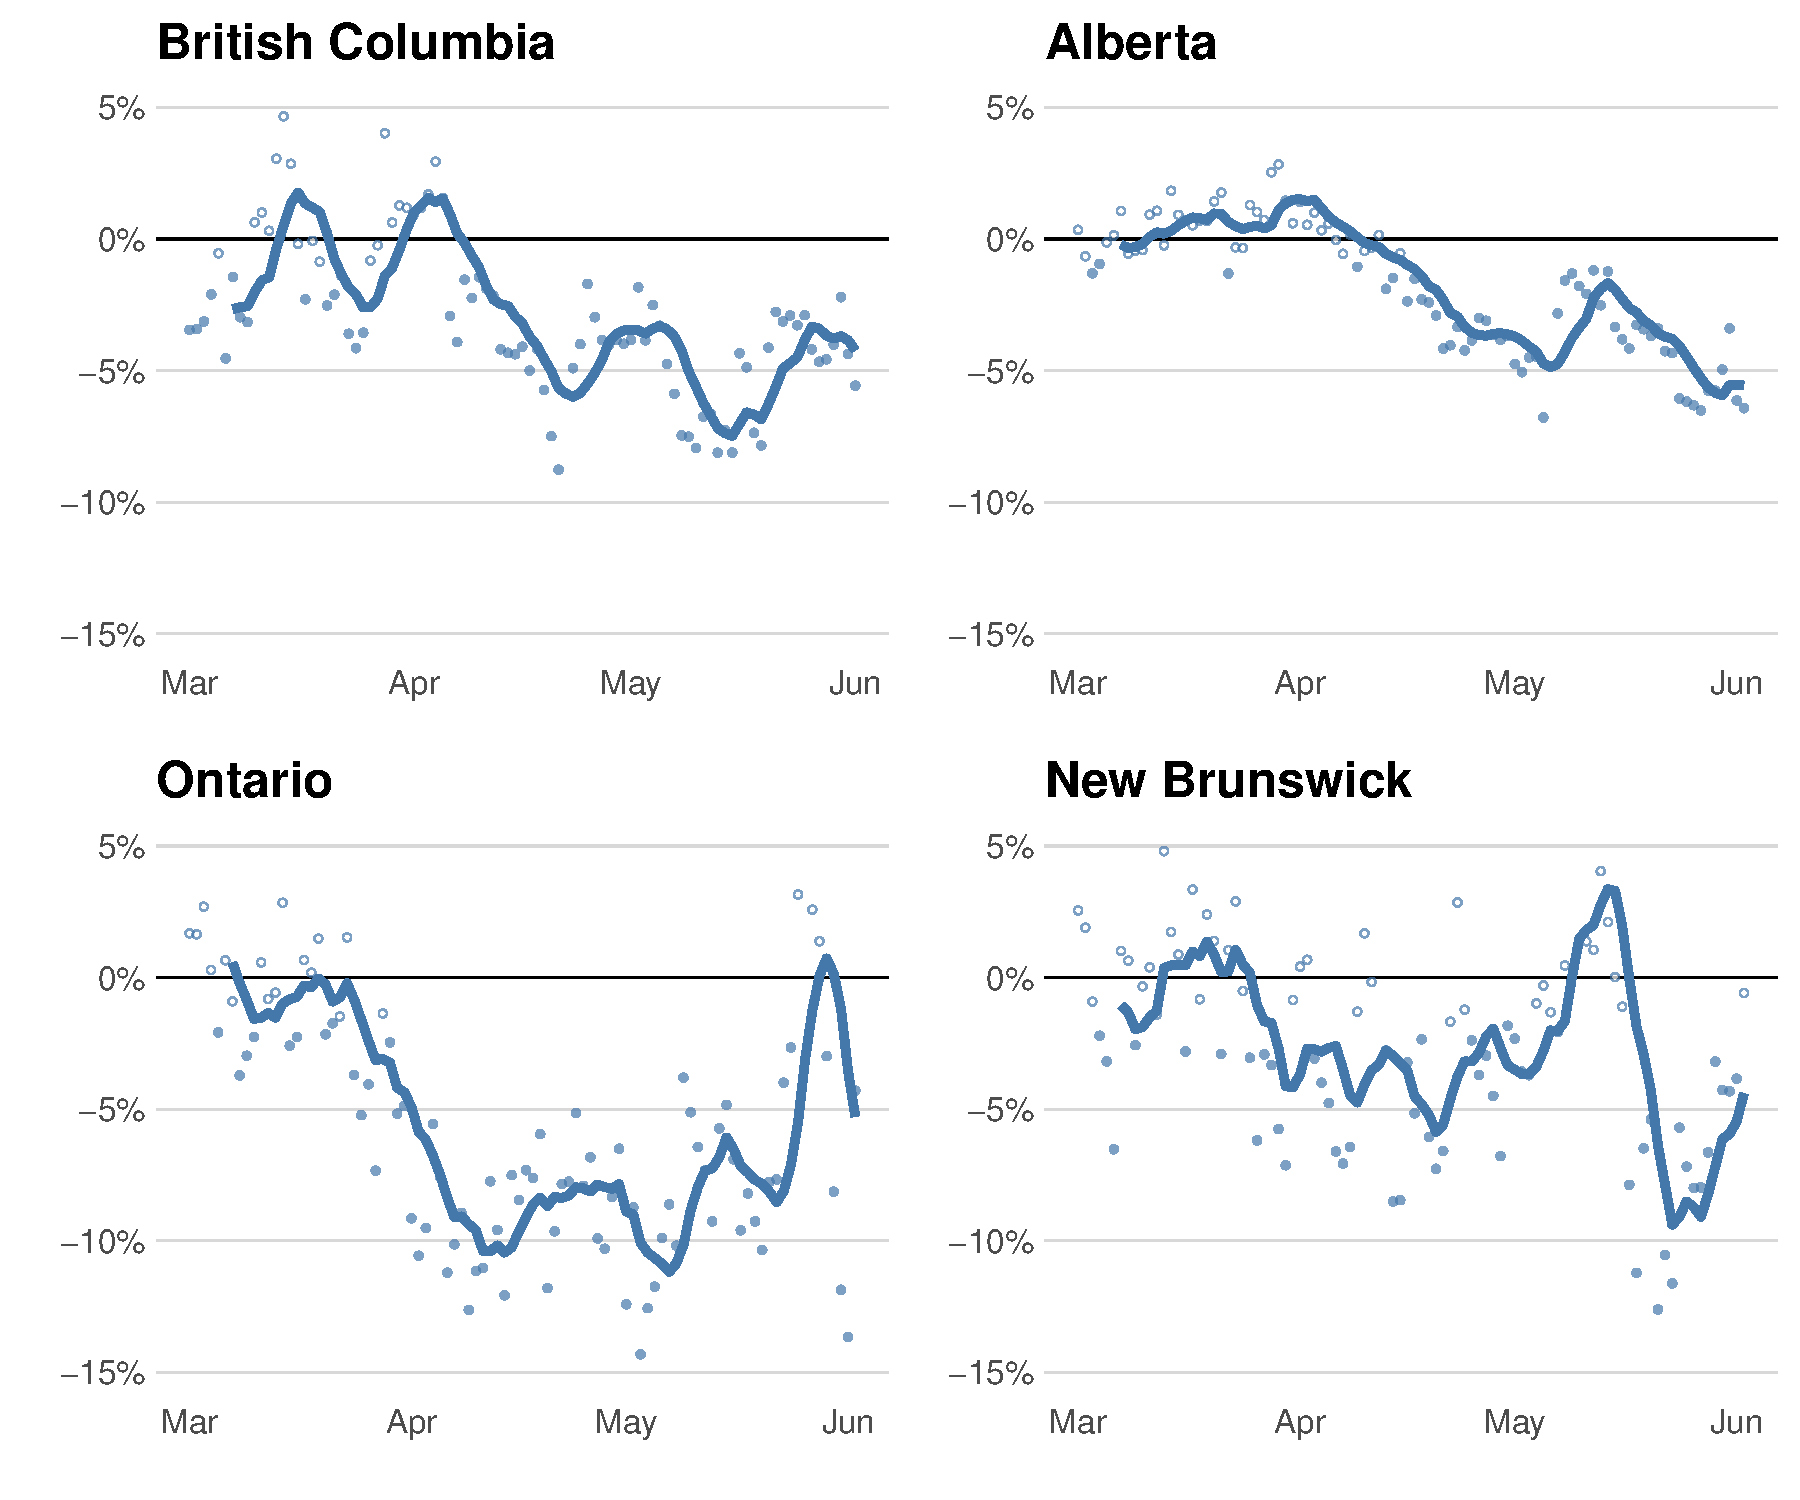
\includegraphics{../images/Fig1.pdf}
\end{frame}

\begin{frame}{Alberta's demand for electricity in COVID Times}
\protect\hypertarget{albertas-demand-for-electricity-in-covid-times}{}
\includegraphics{../images/covid_aeso_fuel.png}
\end{frame}

\begin{frame}{Ontario Industrial demand for electricity in COVID Times}
\protect\hypertarget{ontario-industrial-demand-for-electricity-in-covid-times}{}
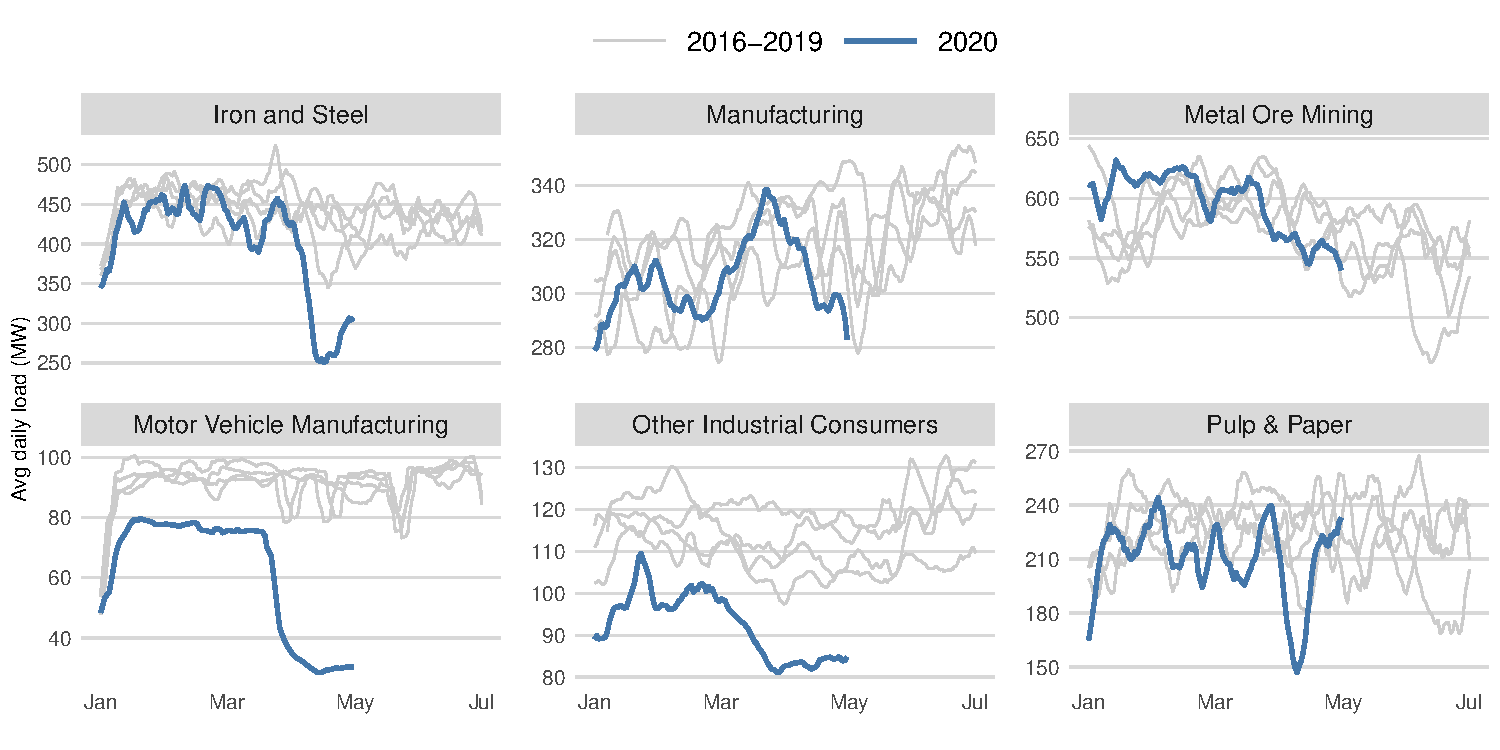
\includegraphics{../images/Fig3.pdf}
\end{frame}


%\section[]{}
%\frame{\small \frametitle{Table of Contents}
%\tableofcontents}
\end{document}
